%!TEX program = xelatex
\documentclass[a4paper, UTF8]{ctexrep}
\usepackage{ctex}
\usepackage{amsmath}
\usepackage{multirow}
\usepackage{amssymb}
\usepackage{graphicx}
\usepackage{geometry}
\usepackage{bm}
\usepackage{subfigure}
\usepackage{float}
\usepackage{array}
\usepackage{makecell}

\renewcommand\thesection{\arabic{section}}

\begin{document}
	\begin{titlepage}
		\centering
		\vspace{6cm}
		\LARGE{\textbf{Deep Learning Homework 1}}\\
		\vspace{4cm}
		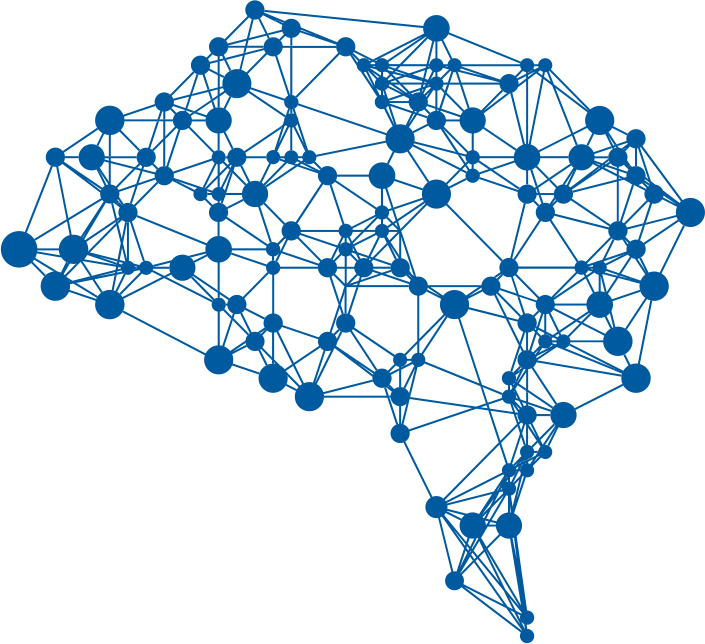
\includegraphics[width=0.8\textwidth]{deepLearning.png}\\
		\vspace{4cm}
		\normalsize{安捷 1601210097}\\
		\normalsize{\today}
	\end{titlepage}
  \section{考虑跨层连接权值的多层BP算法推导}
    由于这一部分公式较多,且为了可以用图示表示清楚推导过程,我用ipad手写了这一部分的推导,本部分内容请看报告最后的附录。
  \section{基于tensorflow的多层感知机(MLP)算法实现}
    我使用python接口的tensorflow库实现了包含一个隐含层的MLP算法,现就算法实现的细节介绍如下:
    \subsection{参数设置}
      \begin{table}[h!]
        \centering
        \begin{tabular}{ccc}
          \hline
          参数名称 & 参数取值 & 参数作用 \\
          \hline
          LAYER\_NUM & 3 & MLP层数 \\
          HIDDEN\_NEURON\_NUM & 500 & 隐含层神经元数目 \\
          TRAIN\_SAMPLE\_NUM & 55000 & 训练数据个数 \\
          TEST\_SAMPLE\_NUM & 10000 & 测试数据个数 \\
          NOLINEAR\_FUNCTION & ReLU & 非线性函数类型 \\
          OPTIMIZER & GradientDescent & 优化函数类型 \\
          BATCH\_NUM & 128 & batch大小 \\
          TRAIN\_CYCLE & 100 & 训练次数 \\
          \hline
        \end{tabular}
        \caption{算法参数表}
      \end{table}
    \subsection{分类准确率}
      经过调参,算法在上述参数表列出的参数下达到准确度:$98.02\%$,重复测试的准确度均为 $98\%$且不随迭代次数增加而增加,同时,增加或减少隐含层节点数目不会提高准确度,可见上述参数设置没有过拟合与欠拟合的情况发生。
    \subsection{代码运行环境及测试平台信息}
      \begin{table}[htbp!]
        \centering
        \begin{tabular}{l}
          \hline
          Python Version: 3.6.0 \\
          Tensorflow Version: tensorflow-gpu-1.0.1 \\
          CUDA Version: 8.0
          OS: Arch Linux \\
          Kernel: x86\_64 Linux 4.10.4-1-ARCH \\
          CPU: Intel Core i7-6700K @ 8x 4.2GHz \\
          GPU: GeForce GTX 1060 6GB \\
          RAM: 16003MiB \\
          \hline
        \end{tabular}
        \caption{代码运行环境及测试环境表}
      \end{table}
      在没有NVIDIA\ GPU及CUDA支持的环境下代码依然可以运行,只是速度较慢
    \section{总结}
      通过这次作业,我学习了tensorflow的基本使用方法,在实现了MLP之后,我又实现了CNN并成功部署到了科研实验中,接下来我将尝试用tensorflow实现FCN用于图像分割;在完成作业的过程中,我同时利用上述测试环境中的CPU与GPU进行了训练,发现GPU训练的速度大约是CPU训练速度的两倍,之后的作业在显存足够的情况下我将主要使用GPU进行训练。
		\section{附录}

\end{document}
